\section{Single Phase Half Wave Controlled Rectifier with R load}

\subsection{Circuit used for simulation}

% figure that is centered on the page
\begin{figure}[h]
    \centering
    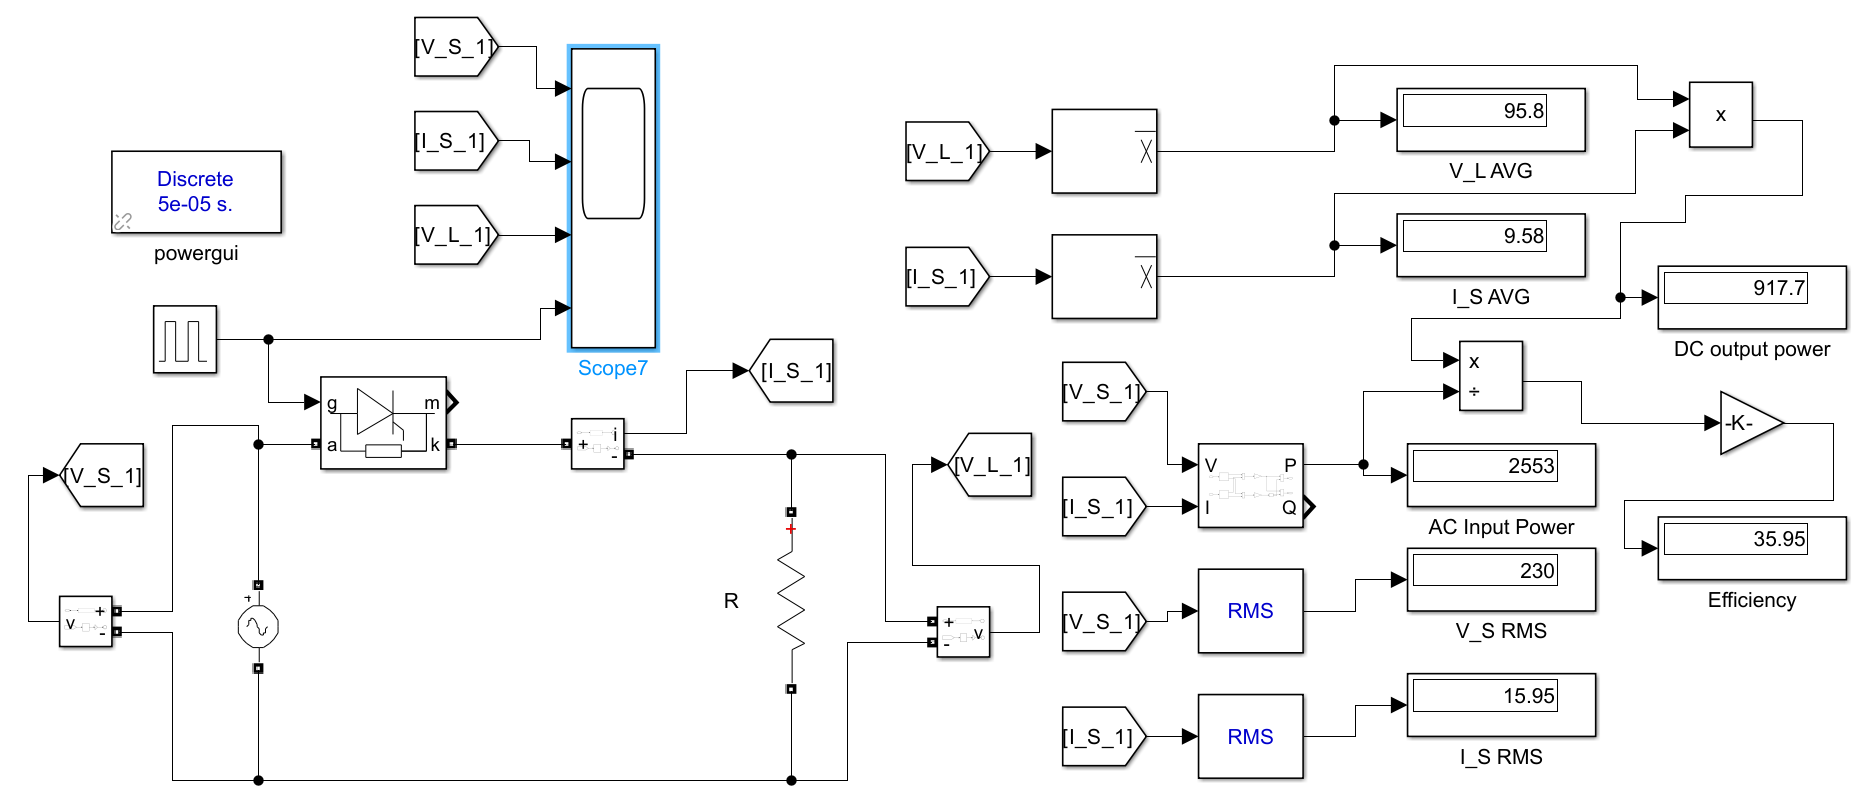
\includegraphics[width=1.0\textwidth]{images/experiment-1/circuit-diagram-experiment-05.png}
    \caption{Circuit for Single Phase Half Wave Controlled Rectifier with R load  (Firing Angle = 30$ ^\circ $)}
    \label{Fig_simulation_circuit_single-phase-half-wave-controlled-rectifier-with-R-load}
\end{figure}

\subsection{Components Required}

\begin{table}[h]
    \renewcommand{\arraystretch}{1.3}
    \label{table_components_required_single-phase-half-wave-controlled-rectifier-with-R-load}
    \centering
    \begin{tabular}{|c|c|c|c|}
        \hline
        Sr. No & Parameters                     & Ratings            & Quantity \\
        \hline
        \hline
        1      & AC Single Phase Voltage Source & 230V ($ V_{rms} $) & 1        \\
        \hline
        2      & Resistor                       & 10$ \Omega $       & 1        \\
        \hline
        3      & Inductor                       & 10mH               & 1        \\
        \hline
        4      & Diode                          & -                  & 1        \\
        \hline
        5      & Voltmeter                      & -                  & 2        \\
        \hline
        6      & Ammeter                        & -                  & 1        \\
        \hline
        7      & Thyristor                      & -                  & 1        \\
        \hline
    \end{tabular}
    \caption{Components for Single Phase Half Wave Controlled Rectifier with R load}

\end{table}



\subsection{Observations}

\begin{table}[h]
    \renewcommand{\arraystretch}{1.3}
    \label{table_observation_single-phase-half-wave-controlled-rectifier-with-R-load}
    \centering
    \begin{tabular}{|c|c|c|}
        \hline
        Parameters                              & Theoretical Values & Simulation Values \\
        \hline
        \hline
        AC Input Voltage ($ V_{in,rms} $)       & 230V               & 230V              \\
        \hline
        Output Average Voltage ($ V_{o,avg} $)  & 96.6V              & 95.8V            \\
        \hline
        Output Average Current ($ I_{o,avg}  $) & 9.66A              & 9.58A            \\
        \hline
        AC Input Power ($ P_{AC}  $)            & 2214.44 (W)        & 2553 (W)          \\
        \hline
        DC Input Power ($ P_{DC}  $)            & 926.98 (W)         & 917.7 (W)         \\
        \hline
        Efficiency (\%)                         & 41.86              & 35.95             \\
        \hline 
    \end{tabular}
    \caption{Observations for Single Phase Half Wave Controlled Rectifier with R load}

\end{table}


The simulation results show that the rectifier circuit is functioning correctly, and the output voltage and current follow the theoretical values closely. As the load is resistive, the output current is in phase with the output voltage. The rectifier circuit is uncontrolled, and the output voltage contains a significant amount of ripple, which can cause problems for some applications.
The efficiency of controlled rectifier with R load is 35.95\%.

\pagebreak


\subsection{Resultant Waveforms}

% figure that is centered on the page
\begin{figure}[h]
    \centering
    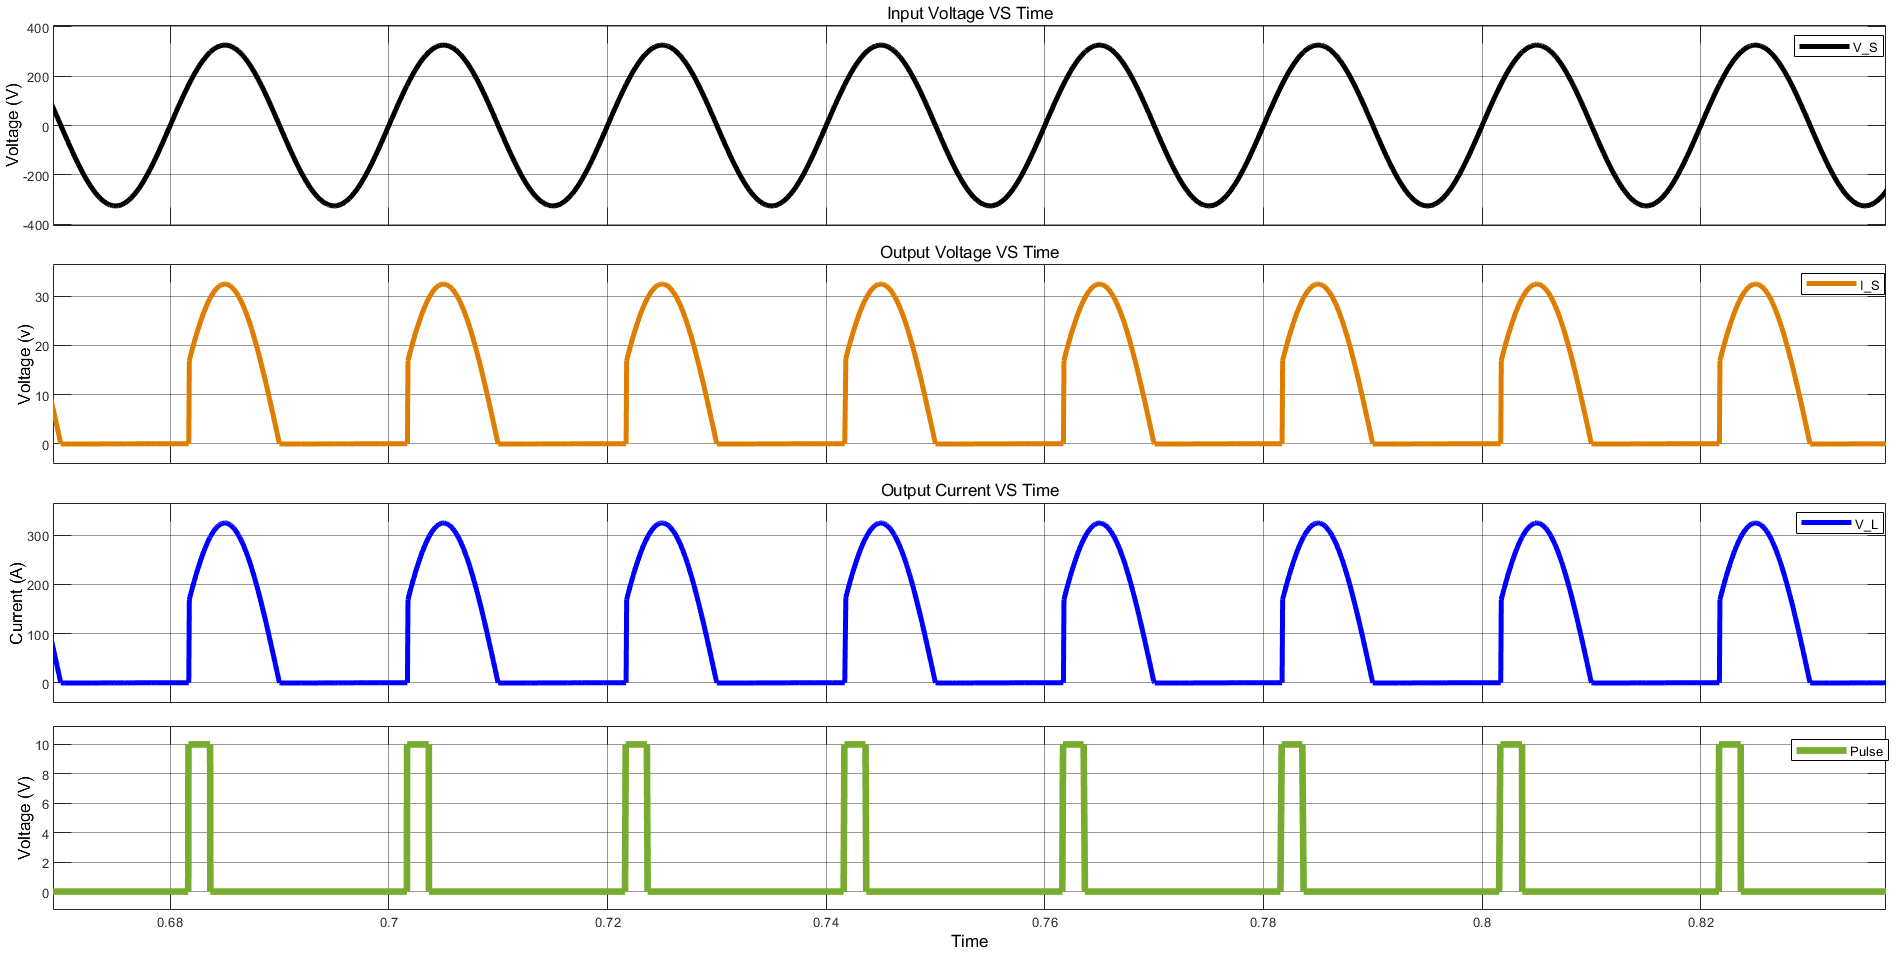
\includegraphics[width=1\textwidth]{images/experiment-1/circuit-scope-experiment-05.png}
    \caption{Scope Waveforms for Single Phase Half Wave Controlled Rectifier with R load}
    \label{Fig_waveform_single-phase-half-wave-controlled-rectifier-with-R-load}
\end{figure}

\pagebreak
